%%%%%%%%                        02 - Práce v týmu                       %%%%%%%%
%---------------------------------------------------------------------------

\begin{frame}
  \frametitle{Práce v týmu}
  \begin{columns}
    \column{1\textwidth}
    \emph{Verzovací systém}
    \begin{itemize}
        \item GitHub
    \end{itemize}
    \emph{Způsob vývoje}
    \begin{itemize}
        \item Pravidelné schůzky 1x do týdne
        \item Rozdělení práce mezi všechny členy týmu na následující týden
    \end{itemize}
  \end{columns}
\end{frame}


%%%%%%%%                       03 - Překladač                      %%%%%%%%
%---------------------------------------------------------------------------


\begin{frame}
  \frametitle{Překladač}
  \tikzstyle{int}=[draw, fill=cyan!12, minimum size=2em]

\begin{tikzpicture}[node distance=4.25cm,auto,>=latex', align=center]
    \node [int] (a) {Zdrojový\\kód\\IFJ21};
    \node [int] (b) [right of=a] {Lexikální\\analyzátor};
    \path[->] (a) edge node {$prog.tl$} (b);
\end{tikzpicture}
\end{frame}

%%%%%%%%                       04 - Lexikální analýza                      %%%%%%%%
%---------------------------------------------------------------------------


\begin{frame}
  \frametitle{Lexikální analýza}
  \begin{columns}
  \column{0.5\textwidth}
  \begin{itemize}
      \item Konečný automat
      \item Přeskočení bílých znaků a komentářů
      \item Vytváření tokenu
  \end{itemize}
  \column{0.5\textwidth}
  \begin{tabular}{ ||c|| } 
      \hline
     token \\ [0.5ex] 
     \hline\hline
     type \\ 
     attribute \\
     \hline
  \end{tabular}\enspace\enspace
  \begin{tabular}{ ||c|| } 
      \hline
     attribute \\ [0.5ex] 
     \hline\hline
     integer \\ 
     decimal \\
     string \\
     keyword \\
     \hline
  \end{tabular}
  
  \end{columns}
\end{frame}

%%%%%%%%                       05 - Lexikální analýza                      %%%%%%%%
%---------------------------------------------------------------------------


\begin{frame}
  \frametitle{Lexikální analýza}
  \begin{columns}
    \column{1\textwidth}
    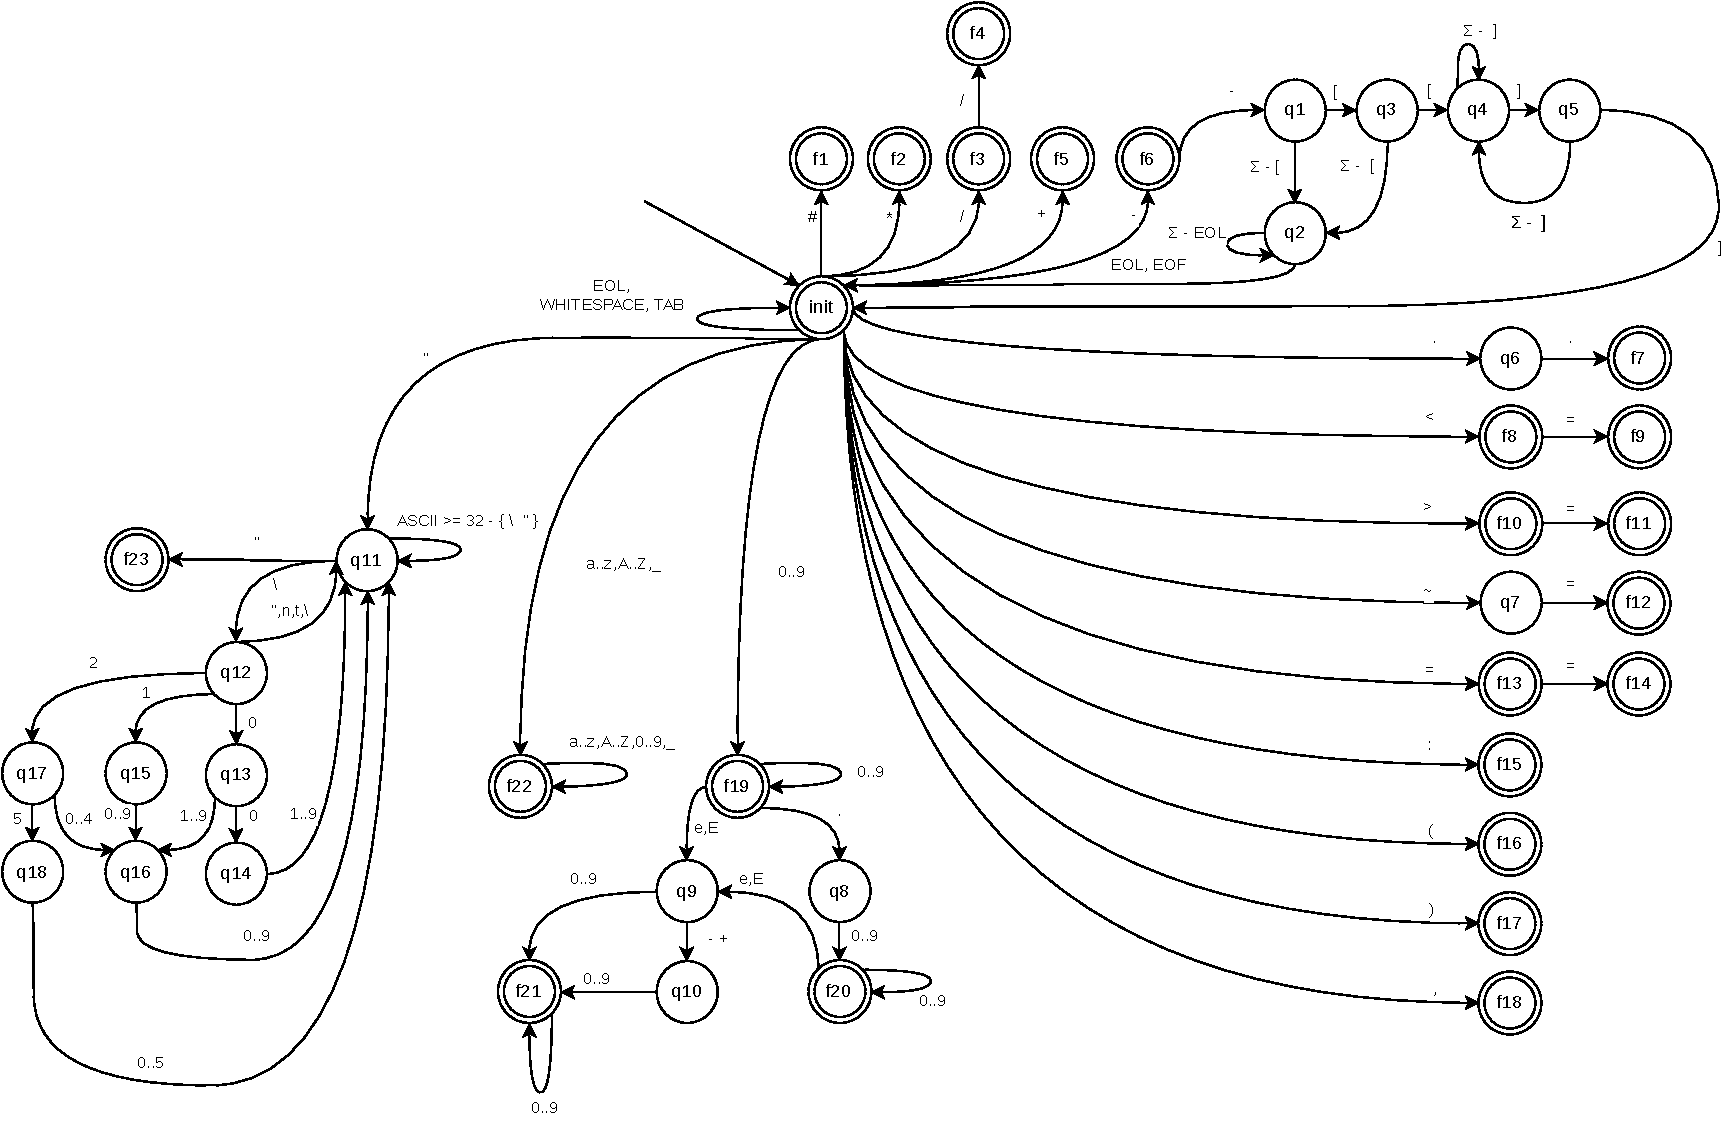
\includegraphics[width=\textwidth]{img/IFJ2021_FSM_final.pdf}
  \end{columns}
\end{frame}

%%%%%%%%                       06 - Překladač                      %%%%%%%%
%---------------------------------------------------------------------------


\begin{frame}
  \frametitle{Překladač}
  \tikzstyle{int}=[draw, fill=cyan!12, minimum size=2em]

\begin{tikzpicture}[node distance=4.25cm,auto,>=latex', align=center]
    \node [int] (a) {Zdrojový\\kód\\IFJ21};
    \node [int] (b) [right of=a] {Lexikální\\analyzátor};
    \node [int] (c) [right of=b] {Syntaktický\\analyzátor};
    \path[->] (a) edge node {$prog.tl$} (b);
    \path[->] (b) edge node {} (c);
\end{tikzpicture}
\end{frame}

%%%%%%%%                       07 - Syntaktická analýza                      %%%%%%%%
%---------------------------------------------------------------------------

\begin{frame}
  \frametitle{Syntaktická analýza}
    \emph{Parser}
    \begin{itemize}
        \item Použitá metoda - Rekurzivní sestup
        \item LL gramatika - 56 pravidel
    \end{itemize}
    \emph{Psa}
    \begin{itemize}
        \item Precedenční tabulka
        \item Gramatika pro výrazy - 15 pravidel
    \end{itemize}
\end{frame}

%%%%%%%%                       08 - Syntaktická analýza                      %%%%%%%%
%---------------------------------------------------------------------------

\begin{frame}
  \frametitle{Syntaktická analýza}
    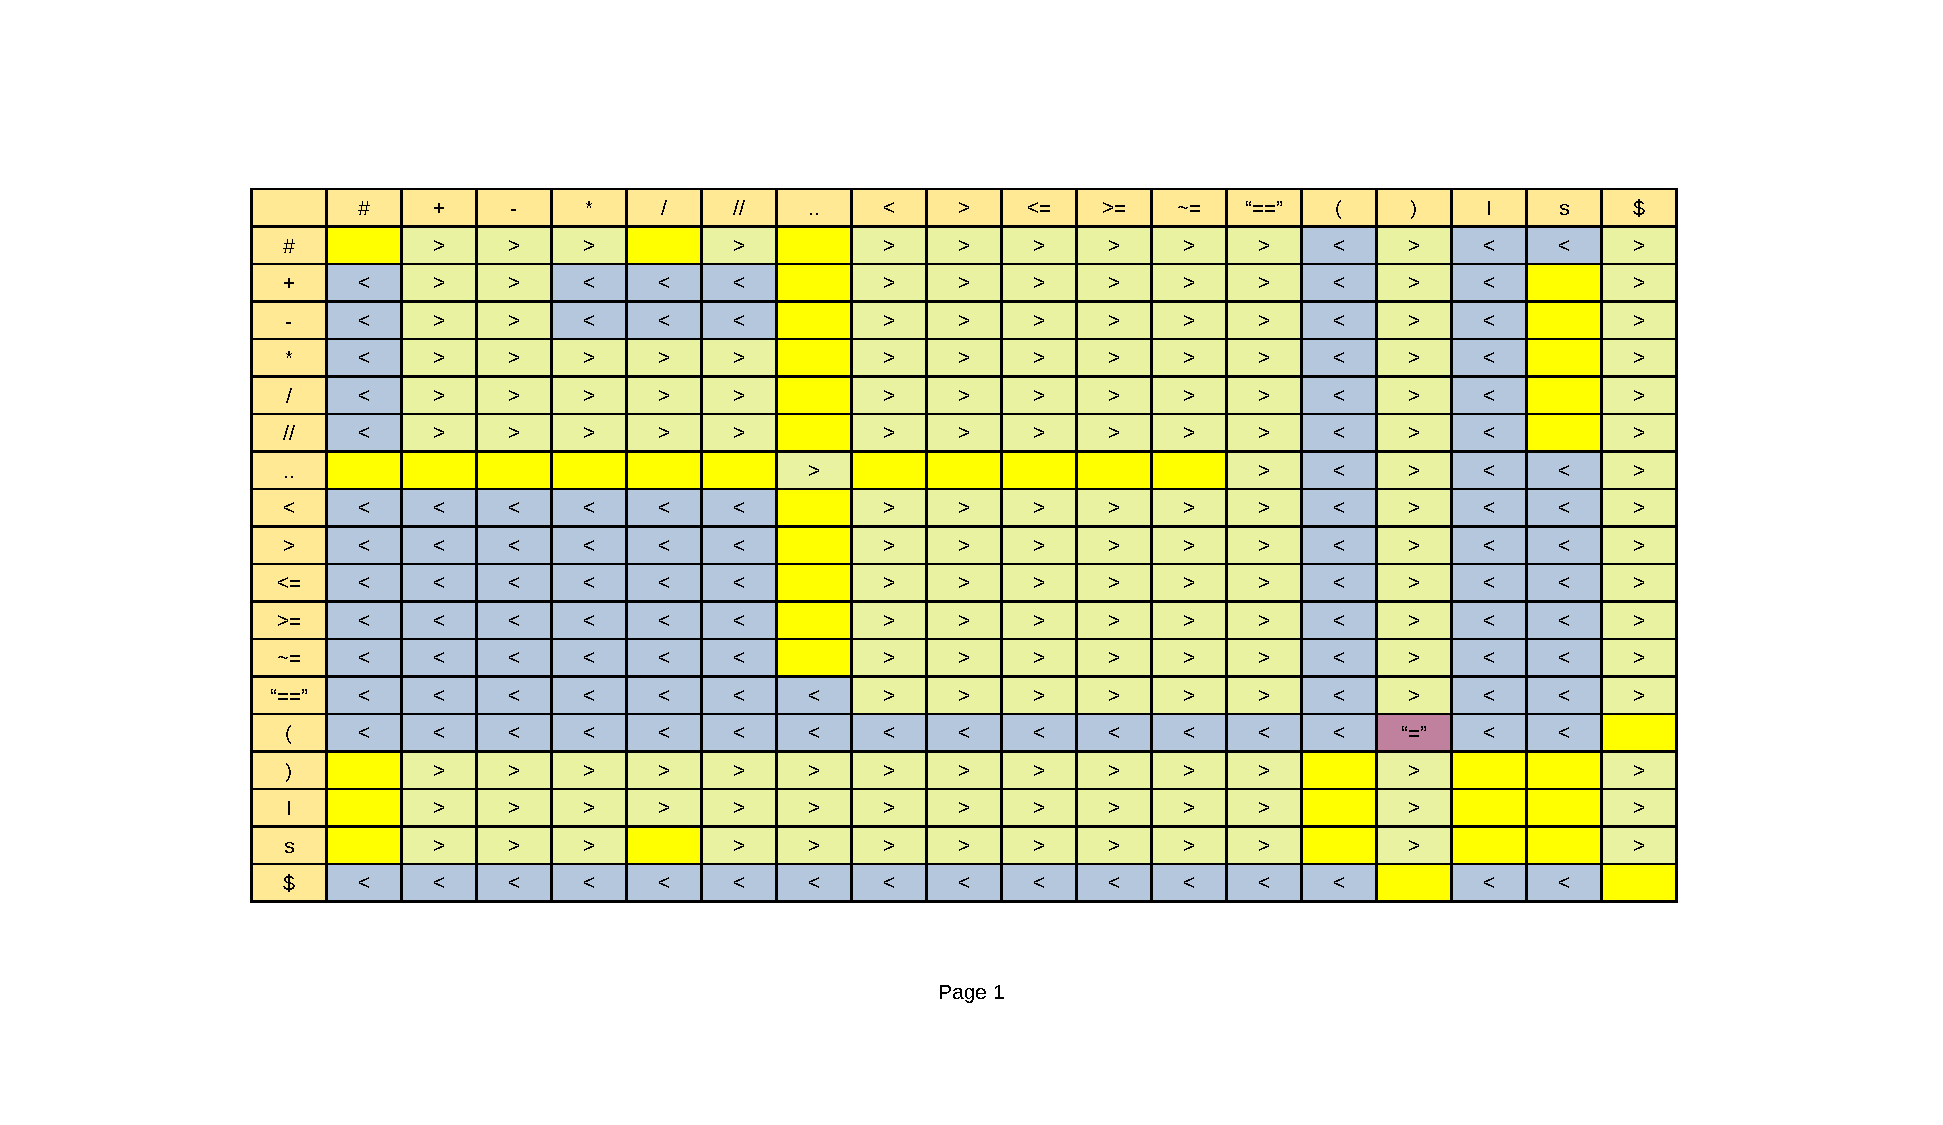
\includegraphics[width=\textwidth, trim={0 2.5cm 0 0},clip]{img/precedence_table.pdf}
    \begin{center}
        \textit{\emph{Precedenční tabulka}}
    \end{center}
\end{frame}

%%%%%%%%                       09 - Překladač                      %%%%%%%%
%---------------------------------------------------------------------------


\begin{frame}
  \frametitle{Překladač}
  \tikzstyle{int}=[draw, fill=cyan!12, minimum size=2em]

\begin{tikzpicture}[node distance=4.25cm,auto,>=latex', align=center]
    \node [int] (a) {Zdrojový\\kód\\IFJ21};
    \node [int] (b) [right of=a] {Lexikální\\analyzátor};
    \node [int] (c) [right of=b] {Syntaktický\\analyzátor};
    \node [int] (d) [below of=c] {Sémantický\\analyzátor};
    \path[->] (a) edge node {$prog.tl$} (b);
    \path[->] (b) edge node {} (c);
    \path[->] (c) edge node {} (d);
\end{tikzpicture}
\end{frame}

%%%%%%%%                       10 - Sémantická analýza                      %%%%%%%%
%---------------------------------------------------------------------------


\begin{frame}
  \frametitle{Sémantická analýza}
  \emph{Parser}
    \begin{itemize}
        \item Využití tabulky symbolů
    \end{itemize}
    \emph{Psa}
    \begin{itemize}
        \item Před redukcí vložení datového typu k symbolu na zásobník
        \item Kontrola kompatibility datových typů
        \item Uložení výsledného datového typu společně s redukovaným neterminálem
    \end{itemize}
\end{frame}

%%%%%%%%                       11 - Tabulka symbolů                      %%%%%%%%
%---------------------------------------------------------------------------


\begin{frame}
  \frametitle{Tabulka symbolů}
    \begin{columns}
  \column{0.5\textwidth}
  \begin{itemize}
      \item Implementace binárním stromem (varianta I)
      \item Neukládání informace o typu identifikátoru (proměnná / funkce)
  \end{itemize}
  \column{0.5\textwidth}
  \begin{tabular}{ ||c|| } 
      \hline
     Element tabulky symbolů \\ [0.5ex] 
     \hline\hline
     declared \\
     defined \\
     data\_type \\
     params\_count \\
     params\_type\_count \\
     returns\_def\_count \\
     returns\_count \\
     first\_param \\
     first\_type\_param \\
     first\_def\_ret \\
     first\_ret \\
     \hline
  \end{tabular}
  \end{columns}
\end{frame}

%%%%%%%%           12 - Jednosměrně vázaný seznam                %%%%%%%%
%---------------------------------------------------------------------------


\begin{frame}
  \frametitle{Jednosměrně vázaný seznam}
    
\begin{tikzpicture}[list/.style={rectangle split, rectangle split parts=2,
    draw, rectangle split horizontal}, >=stealth, start chain]

  \node[list,on chain] (A) {symtable *};
  \node[list,on chain] (B) {symtable *};
  \node[list,on chain] (C) {symtable *};
  \node[on chain,draw,inner sep=6pt] (D) {};
  \draw (D.north east) -- (D.south west);
  \draw (D.north west) -- (D.south east);
  \draw[*->] let \p1 = (A.two), \p2 = (A.center) in (\x1,\y2) -- (B);
  \draw[*->] let \p1 = (B.two), \p2 = (B.center) in (\x1,\y2) -- (C);
  \draw[*->] let \p1 = (C.two), \p2 = (C.center) in (\x1,\y2) -- (D);
\end{tikzpicture}

\tikzset{every tree node/.style={minimum width=2em,draw,circle},
         blank/.style={draw=none},
         edge from parent/.style=
         {draw,edge from parent path={(\tikzparentnode) -- (\tikzchildnode)}},
         level distance=1.5cm}
\begin{tikzpicture}[sibling distance=10pt]
\Tree
[.id1     
    [.id2 ]
    [.id3 
    \edge[blank]; \node[blank]{};
    \edge[]; [.id4
         ]
    ]
]
\end{tikzpicture}
\begin{tikzpicture}[sibling distance=10pt]
\Tree
[.id5     
    [.id6 ]
    [.id7 
    \edge[blank]; \node[blank]{};
    \edge[]; [.id8
         ]
    ]
]
\end{tikzpicture}
\begin{tikzpicture}[sibling distance=15pt]
\Tree
[.f()      
    [.g()  ]
    [.h()  
    \edge[blank]; \node[blank]{};
    \edge[]; [.i()
         ]
    ]
]
\end{tikzpicture}


\end{frame}

%%%%%%%%                       13 - Překladač                      %%%%%%%%
%---------------------------------------------------------------------------


\begin{frame}
  \frametitle{Překladač}
  \tikzstyle{int}=[draw, fill=cyan!12, minimum size=2em]

\begin{tikzpicture}[node distance=4.25cm,auto,>=latex', align=center]
    \node [int] (a) {Zdrojový\\kód\\IFJ21};
    \node [int] (b) [right of=a] {Lexikální\\analyzátor};
    \node [int] (c) [right of=b] {Syntaktický\\analyzátor};
    \node [int] (d) [below of=c] {Sémantický\\analyzátor};
    \node [int] (e) [left of=d] {Generátor\\kódu};
    \path[->] (a) edge node {$prog.tl$} (b);
    \path[->] (b) edge node {} (c);
    \path[->] (c) edge node {} (d);
    \path[->] (d) edge node {} (e);
\end{tikzpicture}
\end{frame}

%%%%%%%%                       14 - Generování kódu                      %%%%%%%%
%---------------------------------------------------------------------------


\begin{frame}
  \frametitle{Generování kódu}
    \emph{Rozhraní}
    \begin{itemize}
        \item Volání funkcí z \textit{codeGen} v těle \textit{parser.c} a \textit{psa.c}
    \end{itemize}
    \emph{Problematika}
    \begin{enumerate}
        \item Deklarace proměnné v cyklu \textit{while}
        \item Stínění proměnných
    \end{enumerate}
    \emph{Řešení}
    \begin{enumerate}
        \item Pomocný \textit{obousměrně vázaný seznam} na odkládání instrukcí
        \item Statická proměnná \textit{scale} a zásobník na ukládání proměnných
    \end{enumerate}
\end{frame}

%%%%%%%%                       15 - Obousměrně vázaný seznam                      %%%%%%%%
%---------------------------------------------------------------------------


\begin{frame}
  \frametitle{Obousměrně vázaný seznam}
    \tikzset{
    squarecross/.style={
        draw, rectangle,minimum size=18pt, fill=orange!80,
        inner sep=0pt, text=black,
        path picture = {
            \draw[black]
            (path picture bounding box.north west) --
            (path picture bounding box.south east)
            (path picture bounding box.south west) --
            (path picture bounding box.north east);
        }
    }
}

\begin{tikzpicture}[
        list/.style={
            very thick, rectangle split,
            rectangle split parts=3, draw,
            rectangle split horizontal, minimum size=18pt,
            inner sep=4pt, text=black,
            rectangle split part fill={blue!20, red!20, blue!20}
        },
        ->, start chain, very thick
      ]

  \node[list,on chain] (A) {\nodepart{second} inst};
  \node[list,on chain] (B) {\nodepart{second} inst};
  \node[list,on chain] (C) {\nodepart{second} inst};

  \node[squarecross]   (D) [right=of C] {};
  \node[squarecross]   (E) [left= of A] {};

  \path[*->] let \p1 = (A.three), \p2 = (A.center) in (\x1,\y2) edge [bend left] ($(B.one)+(0,0.2)$);
  \path[*->] let \p1 = (B.three), \p2 = (B.center) in (\x1,\y2) edge [bend left] ($(C.one)+(0,0.2)$);
  \draw[*->] let \p1 = (C.three), \p2 = (C.center) in (\x1,\y2) -- (D);

  \draw[*->] ($(A.one)+(0.2,0.1)$) -- (E);
  \path[*->] ($(B.one)+(0.1,0.1)$) edge [bend left] ($(A.three)+(0,-0.05)$);
  \path[*->] ($(C.one)+(0.1,0.1)$) edge [bend left] ($(B.three)+(0,-0.05)$);
\end{tikzpicture}
\end{frame}

%%%%%%%%                       16 - Překladač                      %%%%%%%%
%---------------------------------------------------------------------------


\begin{frame}
  \frametitle{Překladač}
  \tikzstyle{int}=[draw, fill=cyan!12, minimum size=2em]

\begin{tikzpicture}[node distance=4.25cm,auto,>=latex', align=center]
    \node [int] (a) {Zdrojový\\kód\\IFJ21};
    \node [int] (b) [right of=a] {Lexikální\\analyzátor};
    \node [int] (c) [right of=b] {Syntaktický\\analyzátor};
    \node [int] (d) [below of=c] {Sémantický\\analyzátor};
    \node [int] (e) [left of=d] {Generátor\\kódu};
    \node [int] (f) [left of=e] {Interpret\\\textit{ic21int}};
    \path[->] (a) edge node {$prog.tl$} (b);
    \path[->] (b) edge node {} (c);
    \path[->] (c) edge node {} (d);
    \path[->] (d) edge node {} (e);
    \path[->] (e) edge node {$prog.code$} (f);
\end{tikzpicture}
\end{frame}

%%%%%%%%                    17 - Výsledky práce                     %%%%%%%%
%---------------------------------------------------------------------------

\begin{frame}
  \frametitle{Výsledky práce}
  \begin{columns}
    \column{1\textwidth}
    \includegraphics[width=\textwidth]{img/tests1.pdf}
  \end{columns}
\end{frame}


%%%%%%%%                    18 - Výsledky práce                     %%%%%%%%
%---------------------------------------------------------------------------

\begin{frame}
  \frametitle{Výsledky práce}
  \begin{columns}
    \column{1\textwidth}
    \includegraphics[width=\textwidth]{img/tests2.pdf}
  \end{columns}
\end{frame}

%%%%%%%%                           Otázky                           %%%%%%%%
%---------------------------------------------------------------------------

\appendix{}
\begin{frame}
  \frametitle{Otázky}
  \begin{center}
    \Large{\emph{Prostor pro dotazy}}
  \end{center}
\end{frame}